\section{Simulation of a Multibody Fleet}\label{sec:test}

We test the collinear predictions on a planar Drake model \cite{tedrake2019drake} of five tugs and one payload (Table~\ref{tab:plant}). The payload is a regular pentagon of circumradius $4$\,m with bow attachments spanning $\pm31.7^\circ$, and each vessel attaches $1.5$\,m astern of its center; parallel cells keep the nominal chords parallel, fan cells spread them over $\pm0.55$\,rad. Each vessel holds its steady-tow thrust open-loop and runs a $50$\,Hz heading loop, proportional in heading error with a cable-bearing trim term; every body receives first-order autoregressive weather with $8$\,s memory. The plant is integrated at $0.5$\,ms. An isolated vessel--payload refinement passes a $0.5$\% energy-envelope criterion at $0.5$\,ms with little margin ($0.47$\%; $0.95$ and $0.23$\% at $1.0$ and $0.25$\,ms) and so selected $0.25$\,ms; the campaign uses $0.5$\,ms for cost, at which the five-vessel engagement peak lies within $0.08$\% of its $0.25$\,ms value. As the cable force is explicit, the error scales with $\omega_e h$ for step $h$, so the $4k$ cells sit at the nominal $1.0$\,ms level. A check declared before its runs re-ran the nominal and $4k$ cells on all 22 seeds at $0.25$\,ms, re-integration of Section~\ref{subsec:magnitude} included: the declared and design-normalized statistics and the interventional swing moved by at most $0.006$ and its lag by under $1$\,ms, each change inside its paired interval and below the half-width of its seed interval.

\begin{table}[t]
  \caption{Testbed Parameters}
  \label{tab:plant}
  \centering
  \setlength{\tabcolsep}{3.4pt}
  \renewcommand{\arraystretch}{0.96}
  \begin{tabular}{llr}
    \toprule
    Quantity & Symbol & Value \\
    \midrule
    Payload mass, drag & $m_L$, $c_L$ & $2500$\,kg, $5500$\,N\,s/m \\
    Vessel mass, drag & $m_A$, $c_A$ & $600$\,kg, $350$\,N\,s/m \\
    Cable stiffness, damping & $k$, $c$ & $1.7\!\times\!10^{5}$\,N/m, $1800$\,N\,s/m \\
    Cable rest length & $L$ & $12$\,m \\
    Payload, vessel yaw inertia & $I_L$, $I_A$ & $2.0\!\times\!10^{4}$, $500$\,kg\,m$^2$ \\
    Payload, vessel yaw drag & & $2.0\!\times\!10^{4}$, $800$\,N\,m\,s \\
    Heading gain (nominal, doubled) & & $500$, $1000$\,N\,m/rad \\
    Cable-bearing trim gain & & $100$\,N\,m \\
    Steady thrust (parallel cells) & $F_T$ & $1.32\,T_0$ \\
    Weather std, payload/vessel & $\sigma_W$ & $3.5$, $0.7$\,kN \\
    Weather memory & $\tau_W$ & $8$\,s \\
    Engagement, payload modes & $\omega_e$, $\omega_L$ & $18.7$, $16.5$\,rad/s \\
    \bottomrule
  \end{tabular}
\end{table}

The campaign has sixteen cells: ten parallel cells spanning $T_0\in\{0.6,1.0,1.4,1.8\}$\,kN, weather intensity $0.5$ or $1$ (Table~\ref{tab:plant} lists intensity 1), and nominal or doubled heading gain; two stiffness cells at $k/4$ and $4k$; and four fan cells. Each cell runs the same 22 seeds, of which 20 are scored; the two pilot seeds, reserved by the declaration for fitting, fit only the neighbor-margin law of the slack-onset test cited in Section~\ref{sec:consequences}. Re-engagements of one cable within $2$\,s of its first form one event, and a scored observation pairs that first re-engagement, with $\Tp\in[T_0,4T_0]$ and all other cables taut, with one neighbor. Drops are read over one engagement period $P=2\pi\sqrt{\mu/k}$, $\mu=m_Am_L/(m_A+m_L)=484$\,kg. Intervals are 95\% bootstraps over whole seeds, with 2000 replicates unless a caption states otherwise.

\subsection{Forecast, Protocol, and Evidence Status}
\label{subsec:forecast}

We committed the forecast and every pass criterion to a hashed declaration \cite{nosek2018preregistration,siepe2024simulation} before launching the campaign and before any neighbor-tension drop had been computed. Ten of the sixteen cells (220 of 352 runs) re-simulate, bit for bit, an earlier campaign on the same seeds, whose stored records (slack-event times and peaks, 1\,Hz tension samples) cannot yield the declared statistic; the forecast has no fitted input. The forecast $R_{ij}$ is the peak tension reduction in cable $i$ per unit half-sine peak applied through cable $j$, from a 34-state translation-invariant linearization of the closed-loop planar fleet about steady tow that retains drag, cable damping, and heading control; the snapping cable contributes only its pulse wrench, and the outputs are $k\,\delta e_i+c\,\delta\dot{e}_i$. Central-difference Jacobians use a step of $10^{-5}$ per reduced coordinate; steps of $10^{-4}$ and $10^{-6}$ change every $R_{ij}$ by less than $10^{-4}$\%.

The declared (pre-registered) window statistic divides the measured tension reduction by $\Tp g_{ij}$, where $g_{ij}$ is the $(i,j)$ entry of $G=(2k/(\omega_L\omega_e))W^\top M_L^{-1}W$ (Section~\ref{sec:model}) divided by \eqref{eq:imp}. At the design geometry of the parallel cells the off-diagonal $g_{ij}$ range from $0.50$ to $1.23$; the statistic instead evaluates $g_{ij}$ at the recorded geometry of each event, where it can approach or cross zero ($g_{ij}\le0$ for $14$--$39$\% of a cell's scored observations). The cell forecast is the median of $R_{ij}/g_{ij}$ over the 20 ordered pairs at the design geometry: $0.165$ in the ten parallel cells at nominal stiffness, $0.139$ and $0.184$ at the stiffness extremes, and $0.176$ in the fan cells. Table~\ref{tab:evidence_status} gives the status of each analysis, that is, when it was specified relative to the data it evaluates.

\begin{table*}[t]
\caption{Evidence Status and Principal Outcomes}
\label{tab:evidence_status}
\centering
\footnotesize
\setlength{\tabcolsep}{3pt}
\renewcommand{\arraystretch}{1.05}
\begin{tabular}{>{\raggedright\arraybackslash}p{2.2cm} >{\raggedright\arraybackslash}p{2.2cm} >{\raggedright\arraybackslash}p{2.9cm} >{\raggedright\arraybackslash}p{5.6cm} >{\raggedright\arraybackslash}p{3.4cm}}
\toprule
\textbf{Analysis} & \textbf{Status} & \textbf{Prediction or benchmark} & \textbf{Observed outcome} & \textbf{Interpretation} \\
\midrule
Impulsive band & Pre-registered & No cell in $[0.2,0.9]$ & None enters; cell medians $0.054$--$0.173$ & Rejects the rigid-impact magnitude \\
Small-peak accuracy & Pre-registered & Ratio to forecast within $\times1.5$, $\Tp<2.3T_0$ & $0.83$--$1.48$ in all 15 evaluable cells & Forecast within declared factor \\
Stiffness trend & Pre-registered & $+0.045$ from $k/4$ to $4k$ & $+0.036$ [$+0.015,+0.058$] & Supports dissipative dependence \\
Pairwise ranking & Pre-registered & Pair order of $R_{ij}$ & Met in 2 of 15 evaluable cells & No pairwise claim \\
Fixed dissipation & Declared addendum & No change, $\gamma$'s fixed & Declared statistic $+0.038$ [$+0.013,+0.060$], a failure; swing (no rule) $+0.007$ [$-0.002,+0.019$] & Statistic responds to geometry; swing flat \\
Second mass ratio & Declared addendum; 18 of 20 seeds blind & Design-normalized $+0.070$ & $+0.065$ [$+0.051,+0.081$]; blind $+0.058$ [$+0.047,+0.081$] & Supports the rise at a second point \\
Magnitude & Post hoc & Committed $0.165$ & Interventional $0.148$ [$0.143,0.154$] ($0.95\times$ forecast per observation; integrator check failed); background-subtracted $0.093$; design-normalized nominal $0.161$ [$0.151,0.167$] & Approximate population magnitude, not a bound \\
\bottomrule
\end{tabular}
\end{table*}

\subsection{Magnitude}\label{subsec:magnitude}

\begin{figure}[t]
  \centering
  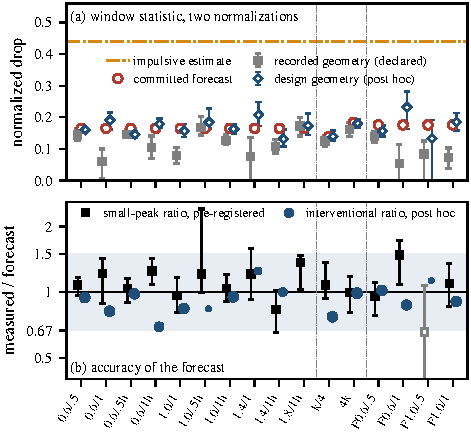
\includegraphics[width=\columnwidth]{fig_cells}
  \caption{Transmission in sixteen cells, labeled by $T_0$ in kN and weather intensity (h: doubled heading gain; F: fan; $k/4$, $4k$: stiffness cells). (a) Declared recorded-geometry statistic (squares) and post hoc design-geometry reading (diamonds), with seed intervals, against the committed forecast (circles). (b) Measured over forecast: pre-registered small-peak ratio (squares, seed intervals; open: unscored cell) and post hoc interventional ratio (circles, area growing with observation count); the band is the declared factor $1.5$.}
  \label{fig:cells}
\end{figure}

The declared statistic stays below the impulsive band $[0.2,0.9]$ in every cell (Fig.~\ref{fig:cells}a) but below the forecast in 14 of 16. On the 3008 re-integrated observations introduced below, an additive background floor ($0.057\Tp$ in time-shifted windows against $0.154\Tp$ at snaps) would raise it; the offset comes instead from the recorded-geometry normalizer, which approaches or crosses zero at re-engagement, and from background motion of either sign inside the window, which can mask the snap response (8\% of those observations record no drop). On them, the drop is $0.80$ times the forecast at the recorded normalizer and $0.99$ at the design normalizer. Applied post hoc, the design normalizer moves the cell medians to $0.132$--$0.232$, putting two cells ($0.208$, $0.232$) inside $[0.2,0.9]$, and the nominal cell ($T_0=0.6$\,kN, intensity $0.5$) from $0.144$ [$0.127,0.163$] to $0.161$ [$0.151,0.167$]; these readings keep the background. For peaks below $2.3T_0$, the pre-registered ratio to the forecast lies within the declared factor $1.5$ in all 15 evaluable cells ($0.83$--$1.48$, Fig.~\ref{fig:cells}b); the fan cell at $T_0=1.0$\,kN, intensity $0.5$, has 12 such observations, below the declared minimum of 20 (unscored ratio $0.66$).

A post hoc estimator, added after the pre-registered verdicts, removes the background: it re-integrates each snap from the recorded state $0.5$\,s before re-engagement under the recorded weather, once as recorded and once without the snapping cable's force, and takes the largest tension difference within one engagement period, on a $10$\,ms grid, per unit $\Tp$ (the interventional swing). It uses a separate $0.5$\,ms semi-implicit Euler model with constant thrust and headings replayed from the record, so the heading loop is not simulated. Its pre-registered check against the record failed on two criteria: other cables' slack onsets over $3$\,s were reproduced for $94.9$\% of 9646 re-engagements against $95$\% ($61$\% in the $4k$ cell, at least $93.8$\% elsewhere), and one grazing contact re-engaged $5.2$\,ms late against a $5$\,ms limit; the median timing error is $6\,\mu$s and the 95th-percentile peak error $0.35$\%. The 3008 observations cover all 22 seeds of four cells and only the two pilot seeds of eleven others (624 from pilots; 2800 at $T_0=0.6$\,kN). Their median swing is $0.148\Tp$ [$0.143,0.154$]; per observation it is $0.95$ times the forecast, and cell medians range from $0.69$ to $1.25$ times it. Subtracting each observation's own time-shifted drop instead (2928 observations with a background window) gives $0.093\Tp$, a lower bound, since background and snap do not add inside a minimum; the gap between the two readings is the width of this measurement.

\begin{figure}[t]
  \centering
  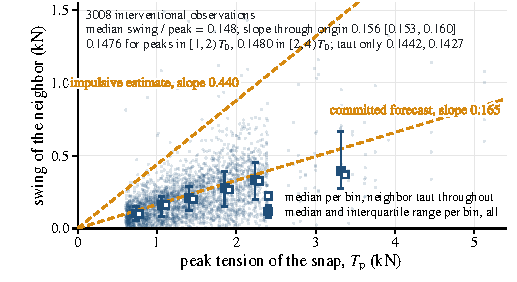
\includegraphics[width=\columnwidth]{fig_swing_vs_peak}
  \caption{Post hoc interventional swing versus snap peak for 3008 observations: medians and interquartile ranges per bin (filled) and medians for the 2766 observations whose neighbor stays taut (open). The through-origin slope is $0.156$ [$0.153,0.160$] (400 bootstrap replicates), versus $0.165$ forecast and $0.440$ impulsively.}
  \label{fig:swingpeak}
\end{figure}

The interventional ratio is $0.1476$ for $\Tp\in[T_0,2T_0)$ and $0.1480$ for $\Tp\in[2T_0,4T_0)$ (Fig.~\ref{fig:swingpeak}), and $0.1442$ and $0.1427$ for neighbors that stay taut, each with a seed interval of $\pm0.005$--$0.008$. They are consistent with, but do not prove, the amplitude invariance of Proposition~\ref{prop:similarity}.

\subsection{Parameter Dependence and Unloading}\label{sec:stiffness}
\begin{figure}[t]
  \centering
  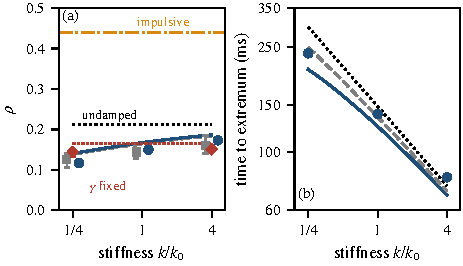
\includegraphics[width=\columnwidth]{fig_stiffness}
  \caption{Stiffness test in the nominal cell. (a) Declared statistic (squares, seed intervals) and post hoc interventional swing (circles) against the dissipative self-consistent (solid) and half-sine (dashed, the committed forecast) models, the undamped law (dotted), and the impulsive estimate (dash-dotted); diamonds: swing on the fixed-dissipation control cells against their flat forecast (red dotted); the control's declared statistic, $0.116$ to $0.154$, which fails that forecast, is not drawn. (b) Time from the snap to the swing's extremum against the same models.}
  \label{fig:stiffness}
\end{figure}

Between $k/4$ and $4k$ the declared statistic rises from $0.125$ to $0.161$, $+0.036$ [$+0.015,+0.058$] over 20 paired seeds, against $+0.045$ predicted and zero from the undamped laws (Fig.~\ref{fig:stiffness}a), the outcome declared as confirming. The median recorded geometry factor is flat in this pair ($0.77$ to $0.78$), so the rise is in the drop itself ($0.135$ to $0.168$ per unit peak). The interventional extremum occurs at $236$, $139$, and $80$\,ms for $k/4$, $k$, and $4k$ (Fig.~\ref{fig:stiffness}b), a ratio of $2.96$ against $2.99$ for the self-consistent model, $3.5$ for the half-sine pulse, and $4$ undamped. That agreement is post hoc: the model times were computed after the measurements, the lags lie on a $10$\,ms grid, and the $k/4$ value rests on 13 snaps from the two pilot seeds.

A control declared before its runs scales $c$, $c_L$, $c_A$ by $\sqrt{k/k_0}$ while varying $k$ (nominal $k_0$), holding $\gamma$, $\gamma_L$, $\gamma_A$ and the linearized forecast fixed at $0.165$. By its declared rule it fails: the declared statistic rises by $+0.038$ [$+0.013,+0.060$]. The rise comes from the normalizer: as the scaled drag changes the shape the fleet holds at re-engagement, the share of observations with $g_{ij}\le0$ falls from $27$ to $16$\% (median $g_{ij}$ $0.69$ to $0.85$), while the drop per unit peak falls from $0.162$ to $0.142$. The interventional swing, declared as a second statistic without an outcome rule, carries neither background nor normalizer and is flat, $0.144$ to $0.151$, $+0.007$ [$-0.002,+0.019$], against $0.117$ (13 pilot snaps) to $0.173$ in the pre-registered pair; its lag ratio is $4.6$ against $4.0$ for the model. On the reading that isolates the transmission, stiffness enters through dissipation, as Proposition~\ref{prop:similarity} states; the declared statistic is also sensitive to the fleet's geometry.

\noindent\textit{Pair structure.}
The post hoc swing improves the rank correlation with $R_{ij}$ in the four fully re-integrated cells ($0.76$, $0.83$, $0.95$ in the parallel cells and $0.47$ in the fan, against $0.24$, $0.21$, $0.58$, $0.31$ for the window drop on the same observations), but the spread of its pair medians within a cell is only $0.054$--$0.067$, against $0.125$--$0.189$ for $R_{ij}$.

\noindent\textit{A second mass ratio.}
A later addendum raised $m_A$ from $600$ to $1250$\,kg ($m_A/m_L=0.50$), for which the collinear model predicts $0.167\to0.238$, printed before the run, and the planar linearization $0.165\to0.234$. It was written after a four-seed pipeline check whose two scored seeds were seen, and its primary statistic is the post hoc design-normalized reading. That statistic rises by $+0.065$ [$+0.051,+0.081$] against $+0.070$ predicted, and by $+0.058$ [$+0.047,+0.081$] on the 18 unseen seeds. The declared secondary statistic, at the recorded geometry, rises by $+0.046$ [$+0.022,+0.073$] ($0.144\to0.189$), and by $+0.038$ [$+0.017,+0.068$] on the unseen seeds; no rule was declared for it.

\noindent\textit{Unloading criterion.}
\begin{figure}[t]
  \centering
  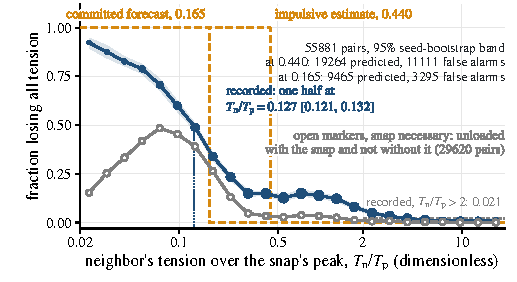
\includegraphics[width=\columnwidth]{fig_threshold_curve}
  \caption{Empirical analog of Corollary~\ref{cor:threshold} over 55\,881 (parent, taut neighbor) pairs. Each candidate $\rho$ is a threshold on $\Tn/\Tp$ (steps); the blue curve (marker area growing with pair count) is the recorded unloading probability with a 400-replicate seed band, crossing one-half at $0.127$ [$0.121,0.132$]. The gray curve (open markers), over 29\,620 re-integrated pairs, is the fraction unloaded in the recorded branch but not the counterfactual one; the dotted level, $0.021$, is the recorded rate at $\Tn/\Tp>2$.}
  \label{fig:threshold}
\end{figure}
Fig.~\ref{fig:threshold} scores $\Tn/\Tp$ over 55\,881 pairs of a declustered parent and a taut neighbor; $19.2$\% unload, and $45.8$\% of the 18\,116 with $\Tp>4T_0$. It is an analog rather than a test of Corollary~\ref{cor:threshold}, which uses $\bar T_{\mathrm p}$ where the figure uses the recorded $\Tp$; the two differ when a neighbor unloads early, as 41\% of unloaded neighbors do within $60$\,ms, near or before the parent's peak. The unloading probability crosses one-half at $0.127$ [$0.121,0.132$]; as classifiers, $\rhoimp=0.440$ recovers 8153 of 10\,735 unloadings with 11\,111 false alarms, and $0.165$ recovers 6170 with 3295. The gray curve counts a neighbor whose elongation crosses zero within $3$\,s in the recorded branch but not in the counterfactual one, the snap as a necessary cause; since the integrator's pre-registered check failed, the declaration requires these counts to be reported as untrusted. It peaks near one-half for $\Tn/\Tp\in[0.05,0.15]$ and is $0.004$ for $\Tn/\Tp>2$ ($0.018$ over all $\Tn/\Tp>0.44$, where neither candidate predicts unloading). The planar transition is therefore population-level, not a deterministic bound on every pair.
